\documentclass[thesis.tex]{subfiles}
\begin{document}
\chapter{Image correspondence}

\section{Dataset}
The dataset we are using for training and evaluation of our descriptor is called the DTU Robot 3D dataset \cite{aanaes2010recall}. It concists of images of objects taken in a black box illuminated using 19 fixed positioned LED lights. In total there are 60 scenes with varying objects. \citet{aanaes2010ground} classify the scenes as shown in \Cref{tbl:dtu_scene_classifications}.

The camera is positioned around each scene using an industrial robot arm, which has automaticly captured each scene from 119 positions. These positions are defined from a fixed frontal view varying the viewpoint $\theta$ in three arcs at different distance $d$ to the scene. Arc 1 has $d = \SI{0.5}{\meter}$ to the scene and $\theta$ spans $\SI{\pm40}{\degree}$, arc 2 has $d = \SI{0.65}{\meter}$ and $\theta$ spans $\SI{\pm25}{\degree}$, and arc 3 has $d = \SI{0.8}{\meter}$ and $\theta$ spans $\SI{\pm20}{\degree}$. Furthermore a linear path is captured by moving the camera away from the scene, which corresponds to zooming or scaling the scene. This is done at $\theta = \SI{0}{\degree}$ and $d$ spans $[\SI{0.5}{\meter};\SI{0.8}{\meter} ]$. At each of the 119 camera positions 19 individual images $I_i$ are taken with each of the LED lights $i,~\text{for}~i = 1,\hdots,19$ turned on. Using the given camera positions we get four camera paths: three arc paths and one linear path.

\todo{Create appropriate figure of arcs, linear- and light paths}

The choice of capturing the scenes with individual LED lights created images with a high amount of casting shadows. We therefore create artificial diffuse light images from the individual lightings in order to only evaluate the performance of our descriptor under viewpoint changes and to get more natural images. These diffuse images are created by averaging over the individual light images for each camera position:
\begin{align}
	I_{\text{diffuse}} = \frac{1}{19} \sum_{i = 1}^{19} I_{i}
\end{align}
Since we have individual LED images we are able to construct images simulating two light source paths going from right to left and back to front respectively.
Given a light position $L_{\boldsymbol{x}}$ in the spatial domain of the LED positions, the image $I_{\boldsymbol{x}}$ is constructed by weighting each LED image by the Gaussian of the distance to $L_{\boldsymbol{x}}$:
\begin{align}
	L_{x} = \sum_{i = 1}^{19} G(\boldsymbol{x} - \boldsymbol{x}_i,\sigma) I_{i}
\end{align}
See \citet{aanaes2010ground} for more information about the dataset and the generated light paths.


\Cref{fig:light_example} show 6 of the different light images for scene 4 at camera position 60. \Cref{fig:light_example_02,fig:light_example_17,fig:light_example_08} show the images taken with individual LED lighting (numbers 2, 17, and 8 respectively), and \Cref{fig:light_example_00} shows the diffuse light image. We here notice the significant difference in cast shadows using the three LEDs individually compared to the diffuse light image. The diffuse light image is however quite dark compared to the LED 8 light image, which could potentially cause problems in some scenes generating too few interest points. Such an issue could however be handled by adapting detection thresholds.
\Cref{fig:light_example_28,fig:light_example_20} show the left- and rightmost positions of the X light path. By comparing these to their LED counterparts (\subref{fig:light_example_02} and \subref{fig:light_example_17} respectively) we see that the cast shadows are less significant therefore looking more natural.
\Cref{fig:viewpoint_example} shows 4 different camera positions for scene 4 including the keyframe (position 25).
\mycomment[MSN]{Should we write a notice about errorneous cast shadows (001-01\_03), and what else for viewpoint example?}
%
\begin{figure}[ht]
	\centering
	\begin{subfigure}{0.49\textwidth}
		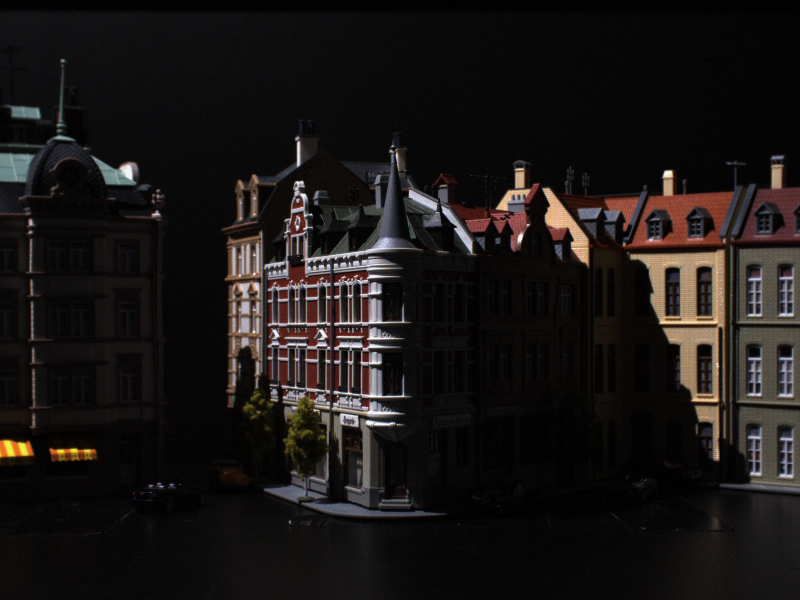
\includegraphics[width=\textwidth]{img/scene_04_img60_02.png}
		\caption{LED 2 light}
		\label{fig:light_example_02}
	\end{subfigure}
	\begin{subfigure}{0.49\textwidth}
		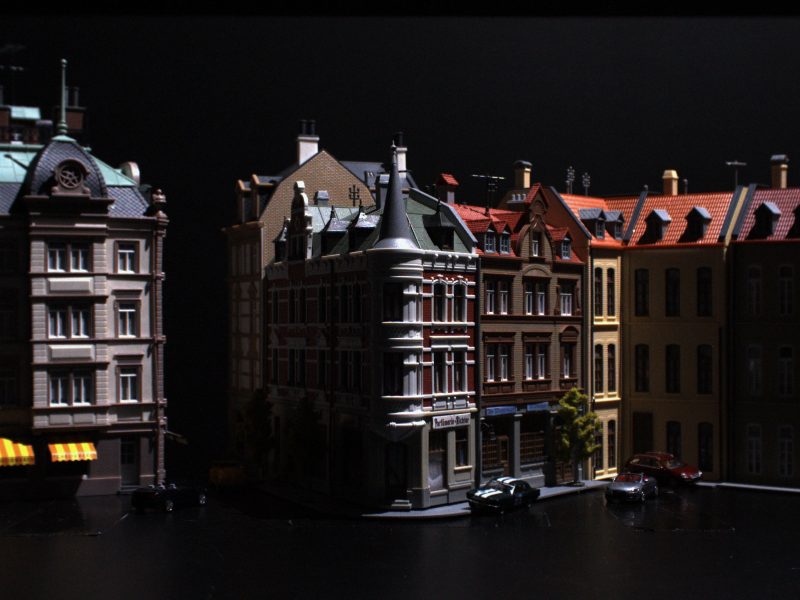
\includegraphics[width=\textwidth]{img/scene_04_img60_17.png}
		\caption{LED 17 light}
		\label{fig:light_example_17}
		\end{subfigure}
	\begin{subfigure}{0.49\textwidth}
		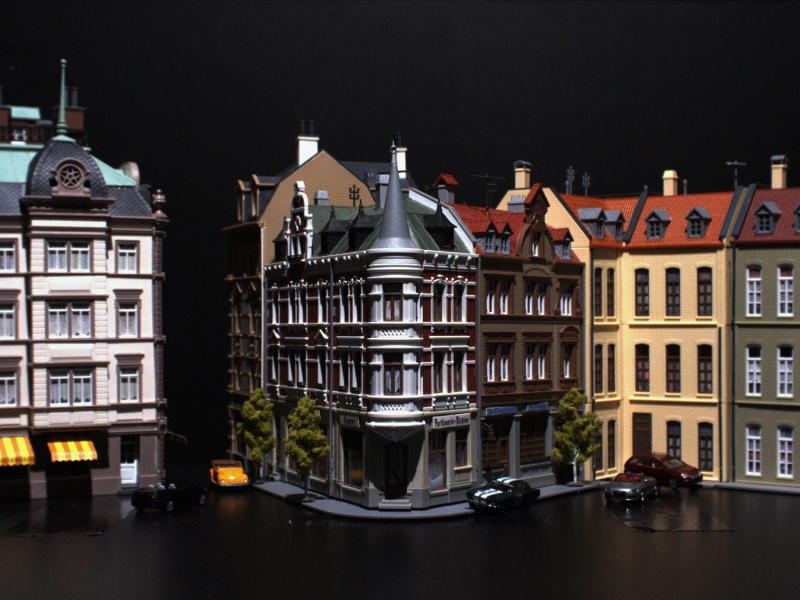
\includegraphics[width=\textwidth]{img/scene_04_img60_08.png}
		\caption{LED 8 light}
		\label{fig:light_example_08}
	\end{subfigure}
	\begin{subfigure}{0.49\textwidth}
		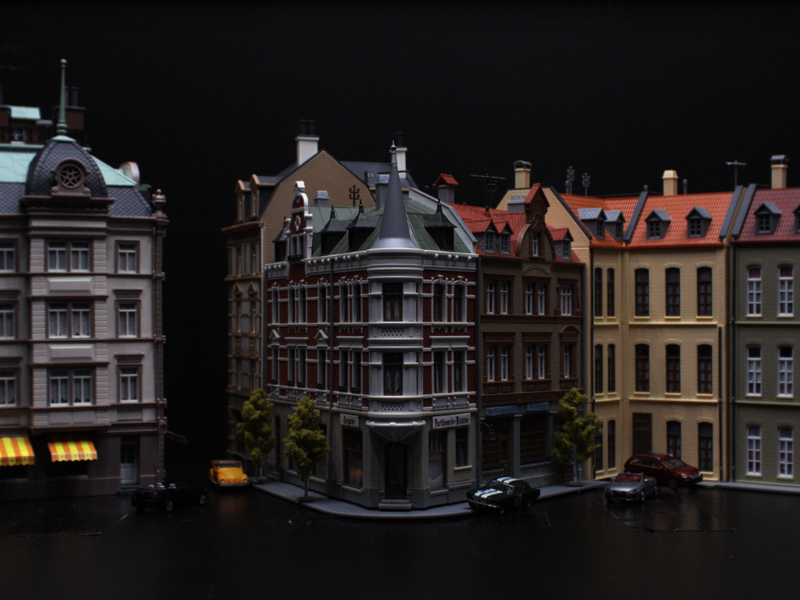
\includegraphics[width=\textwidth]{img/scene_04_img60_00.png}
		\caption{Diffuse light}
		\label{fig:light_example_00}
	\end{subfigure}
	\begin{subfigure}{0.49\textwidth}
		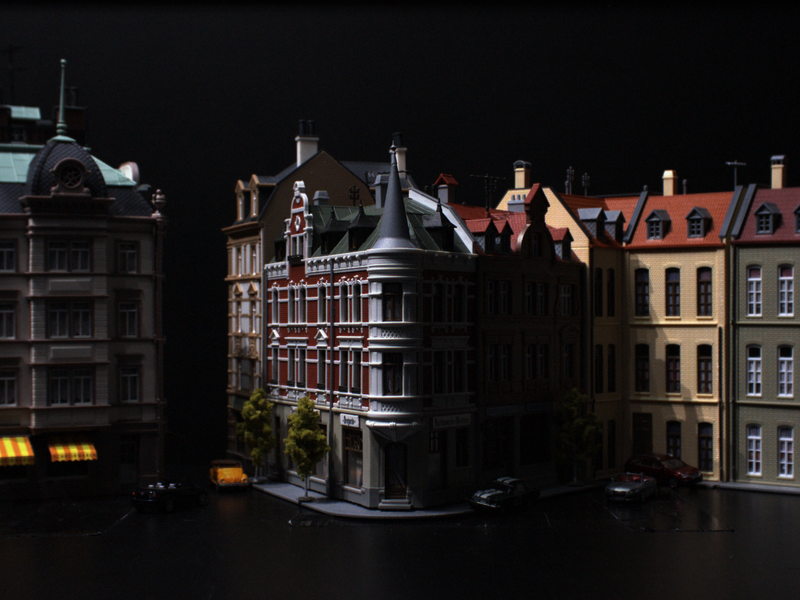
\includegraphics[width=\textwidth]{img/scene_04_img60_28.png}
		\caption{Leftmost position of X light path}
		\label{fig:light_example_28}
	\end{subfigure}
	\begin{subfigure}{0.49\textwidth}
		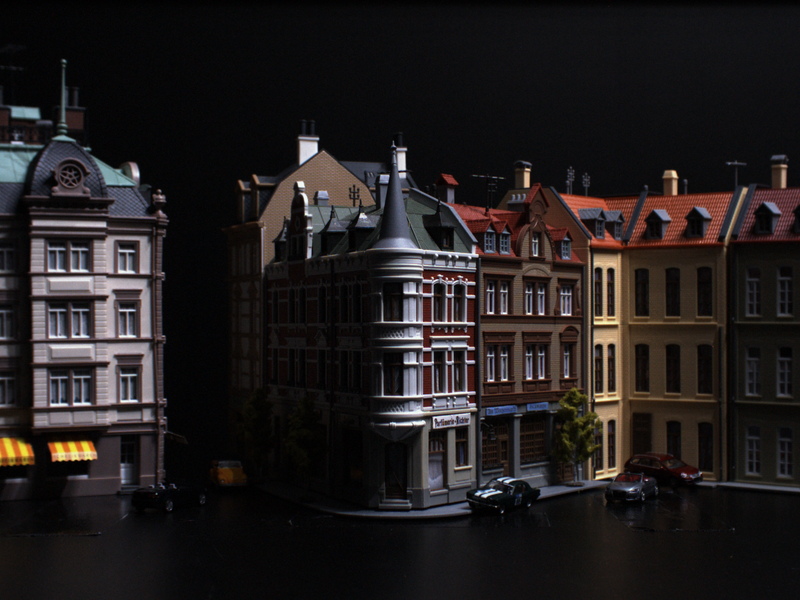
\includegraphics[width=\textwidth]{img/scene_04_img60_20.png}
		\caption{Rightmost position of X light path}
		\label{fig:light_example_20}
	\end{subfigure}
	\caption{Examples of light images in scene 4 at camera position 60.}
	\label{fig:light_example}
\end{figure}
%
\begin{figure}[ht]
	\centering
	\begin{subfigure}{0.49\textwidth}
		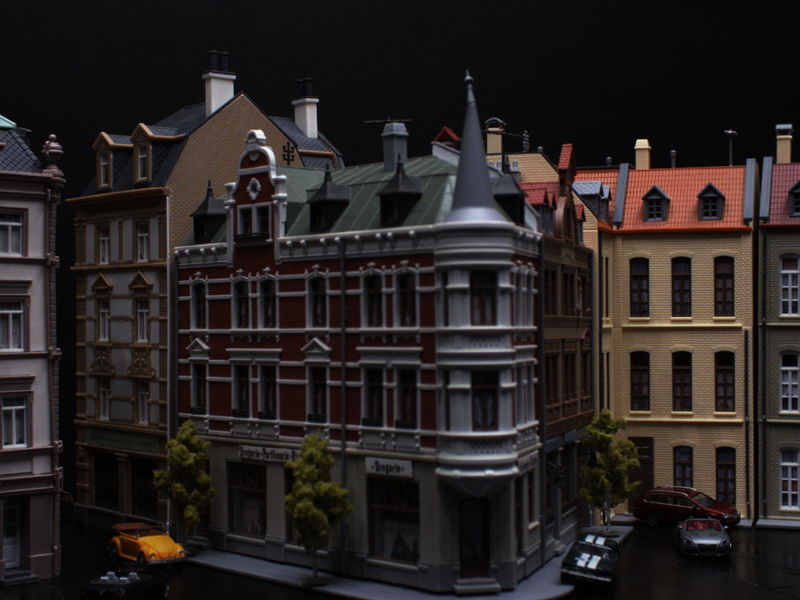
\includegraphics[width=\textwidth]{img/scene_04_img12_00.png}
		\caption{Camera position 12 (arc 1)}
		\label{fig:viewpoint_example_left}
	\end{subfigure}
	\begin{subfigure}{0.49\textwidth}
		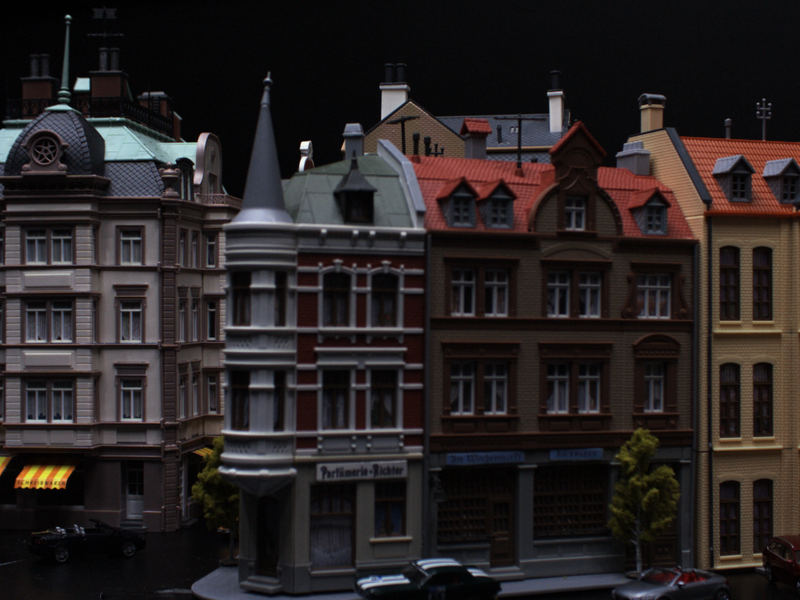
\includegraphics[width=\textwidth]{img/scene_04_img47_00.png}
		\caption{Camera position 47 (arc 1)}
		\label{fig:viewpoint_example_right}
	\end{subfigure}
	\begin{subfigure}{0.49\textwidth}
		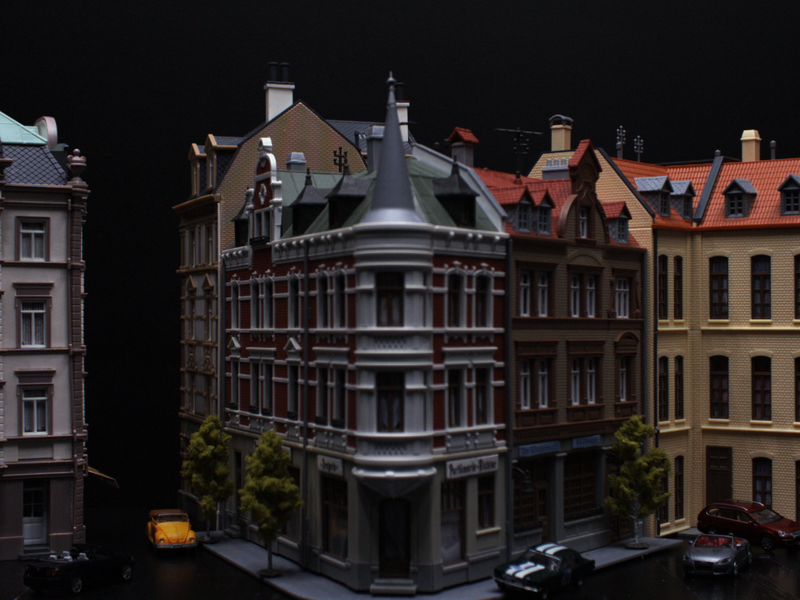
\includegraphics[width=\textwidth]{img/scene_04_img25_00.png}
		\caption{Camera position 25 (keyframe)}
		\label{fig:viewpoint_example_keyframe}
	\end{subfigure}
	\begin{subfigure}{0.49\textwidth}
		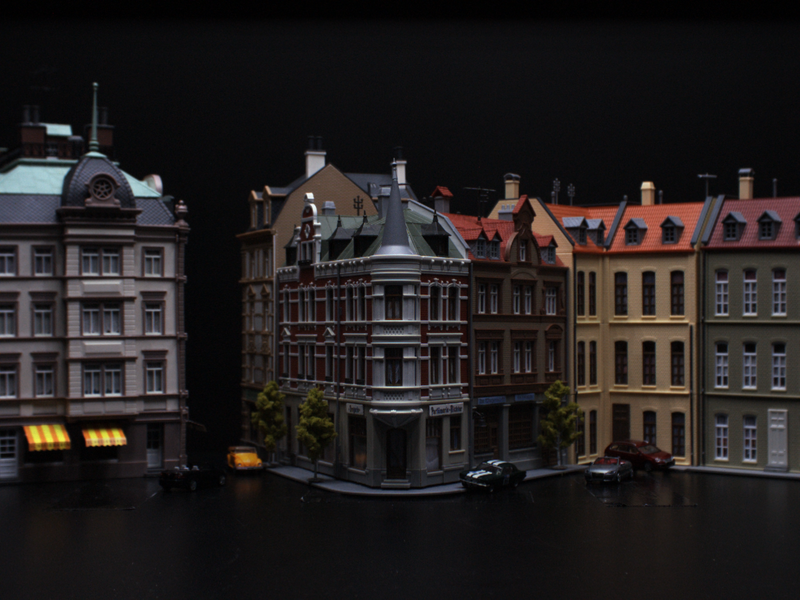
\includegraphics[width=\textwidth]{img/scene_04_img64_00.png}
		\caption{Camera position 64 (linear path)}
		\label{fig:viewpoint_example_scale}
	\end{subfigure}
	\caption{Examples of various camera positions of scene 4 using diffuse light.}
	\label{fig:viewpoint_example}
\end{figure}
%
\begin{table}[ht]
	\centering
	\begin{tabular}{l l r}
		\toprule
		Class & Scene numbers & Total \\
		\midrule
		House					& 1, 4, 8, 31, 32, 49, 50, 55				& 8 \\
		Books					& 2, 11, 20, 21								& 4 \\
		Fabric					& 5, 6, 45, 46, 47, 48						& 6 \\
		Greens					& 23, 24, 25, 26, 27, 51, 52, 53, 54, 56	& 10 \\
		Beer  					& 15, 16									& 2 \\
		Teddy Bears 			& 9, 10, 43, 44								& 4 \\
		Building Materials 		& 33, 34, 35, 36, 37						& 5 \\
		Decorative Items (Art) 	& 38, 39, 40, 41, 42						& 5 \\
		Groceries 				& 12, 28, 29, 30							& 4 \\
		Twigs and Leaves 		& 17, 57, 58, 59, 60 						& 5 \\
		\bottomrule
	\end{tabular}
	\caption{Scene object classifications from \cite[Table 1]{aanaes2010ground}}
	\label{tbl:dtu_scene_classifications}
\end{table}
%
\section{Experiments}


\section{Parameter study}



Test: 10 fold cross validation

\section{Evaluation}


\subbibliography

\end{document}
